\section{Sombreado de Vóxeles} % (fold)
\label{sec:sombreado_de_voxeles}
Para el cálculo de iluminación indirecta es necesario sombrear cada vóxel. El proceso de sombreado de vóxeles nos permite almacenar la radiancia incidente sobre la escena discretizada en vóxeles. En el trabajo de Crassin esto se hace calculando la iluminación directa sobre los vóxeles utilizando \emph{light-view maps} por cada fuente de luz como ya fue explicado en la sección \ref{subsub:voxel_capture}. Este proceso puede ser ineficiente tanto en consumo de memoria como en rendimiento cuando se considera una escena con muchas luces ya que por cada luz se debe realizar este proceso y se debe tener un mapa de luz-vista asociado (seis para luces puntuales). Otra desventaja de este método es la dependencia del rendimiento con la resolución del mapa de luz-vista. Al aumentar la resolución de esta textura también se aumenta el número de colisiones por cada fragmento que desear escribir sobre un mismo vóxel.

Nuestra implementación utiliza \emph{compute shaders} o el procesador de computo en la \ac{GPU} para el sombreado difuso de cada vóxel. Para calcular el termino difuso sobre un fragmento utilizando la \ac{BRDF} de Lambert (ecuación \ref{eq:lambert}) necesitamos saber el valor de $\rho_{d}$ el cual ya es almacenado en nuestro volumen albedo. Esta constante luego debe ser multiplicada por el $\cos(N_{x}, \Psi)$ para calcular la reflexión difusa de este fragmento. Por esto también se crea un volumen de normales. El vector $\Psi$ se obtiene a partir la dirección de cada fuente de luz en escena.

Para fuentes de luz con dirección no uniforme como luces puntuales o focales es además necesario saber la posición de este fragmento. Siendo cada vóxel una representación discreta de un espacio en escena almacenado en una textura 3D, esta posición se extrae fácilmente convirtiendo la posición tridimensional del vóxel en espacio textura a su equivalente en espacio de mundo.

Al promediar las normales en el espacio de un vóxel pueden surgir varios problemas de precisión. Esto sucede especialmente cuando un vóxel envuelve superficies finas cercanas con normales opuestas. Para solventar este problema se implementaron dos modelos de iluminación de vóxeles. El modelo de Lambert clásico utilizando la normal promedio del vóxel directamente y otro modelo al cual llamaremos Lambert Direccional Ponderado donde se calcula la reflexión difusa por cada cara del vóxel para luego promediar este resultado según el peso de cada eje en el vector normal promedio.

\begin{figure}[H]
	\centering
	\begin{subfigure}[t]{0.33\textwidth}
		\centering
		\captionsetup{justification=centering}
		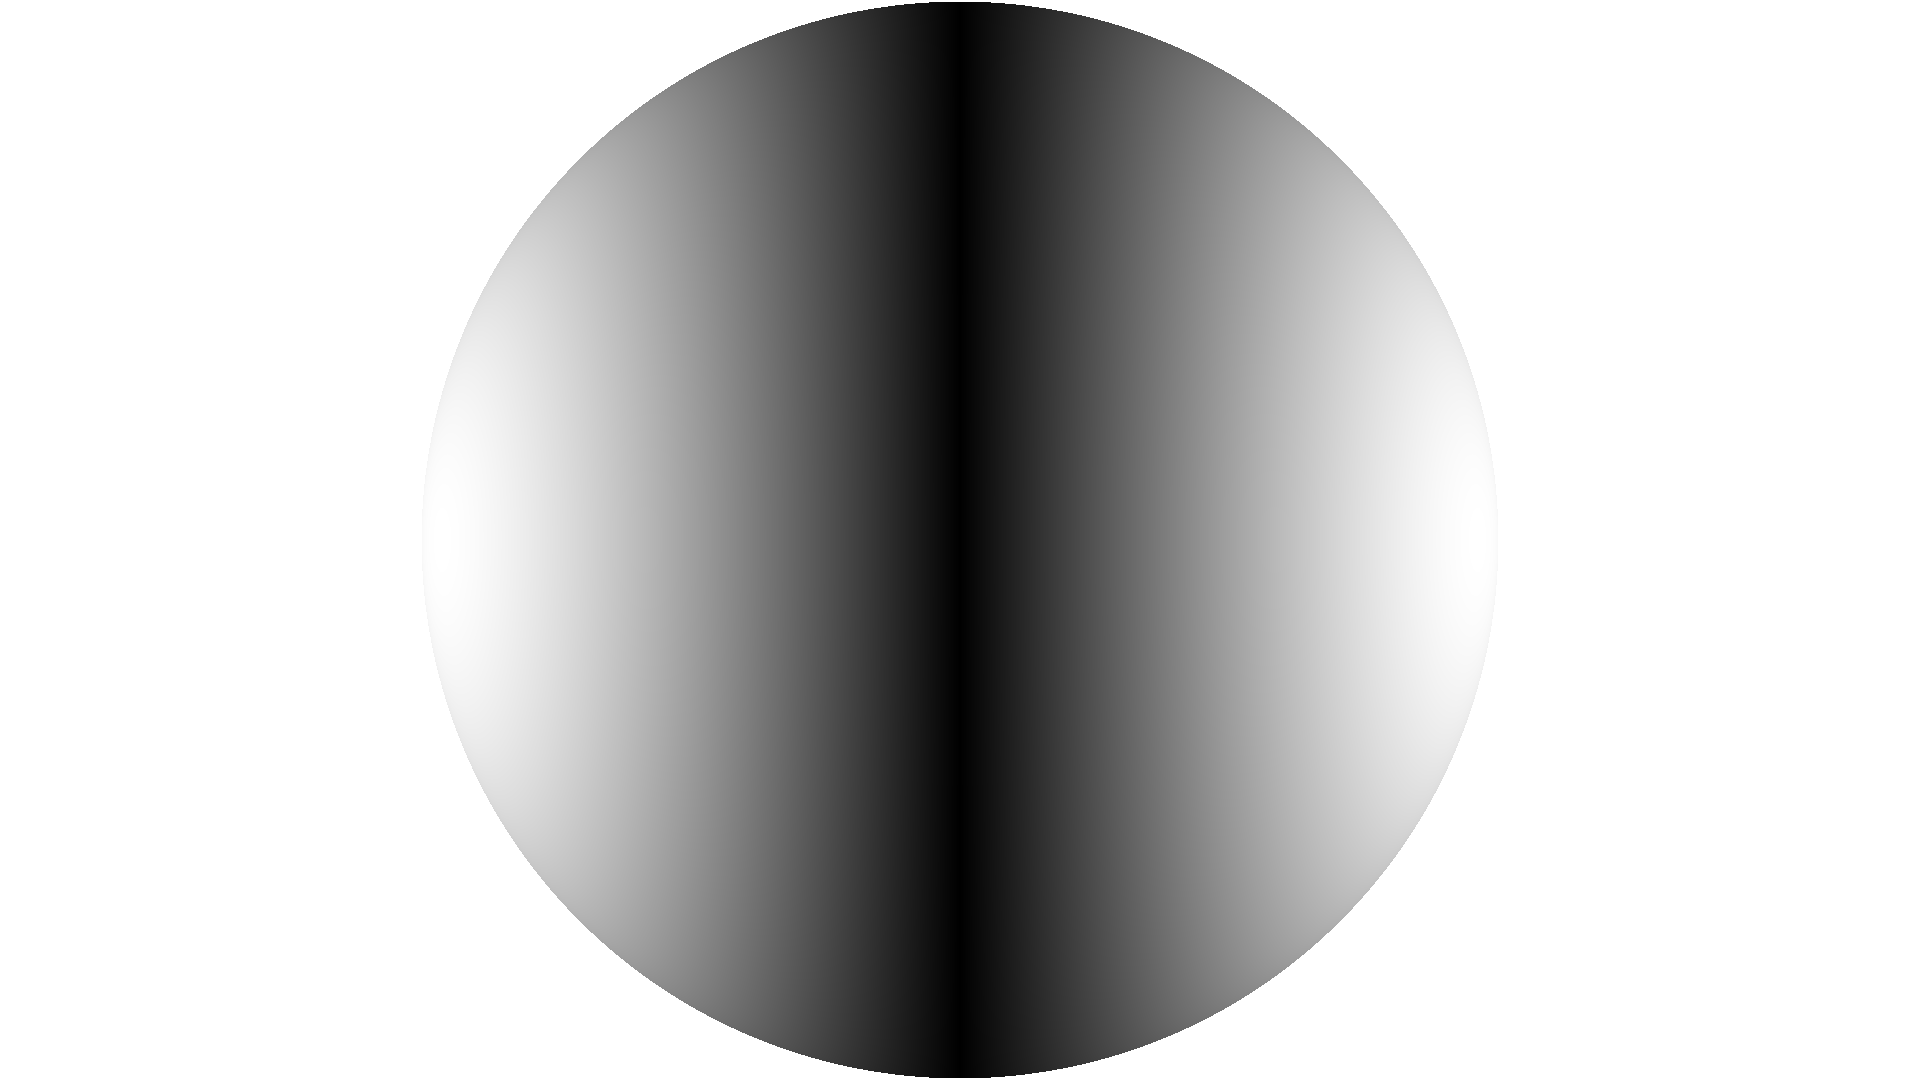
\includegraphics[width=\linewidth]{media/lambert_right.png}
		\caption*{Eje x.}
	\end{subfigure}%
	\begin{subfigure}[t]{0.33\textwidth}
		\centering
		\captionsetup{justification=centering}
		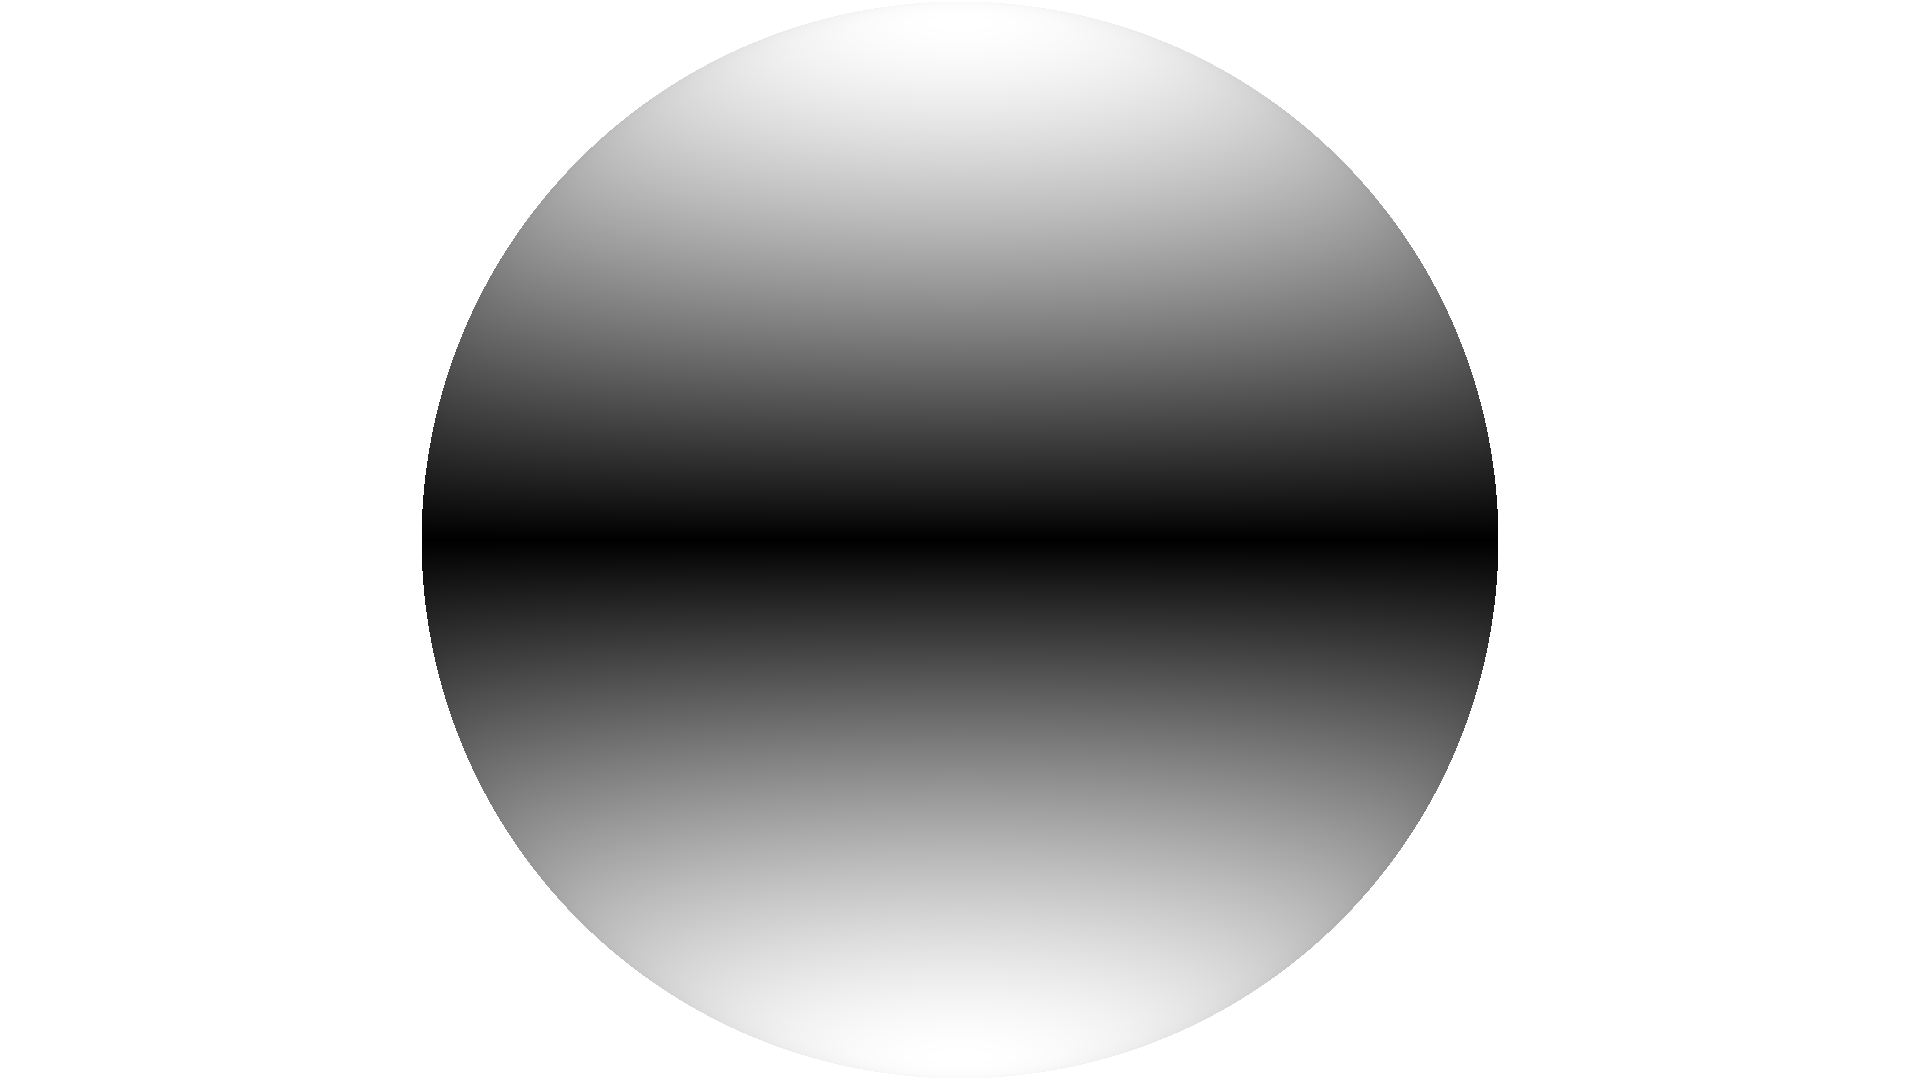
\includegraphics[width=\linewidth]{media/lambert_up.png}
		\caption*{Eje y.}
	\end{subfigure}%
	\begin{subfigure}[t]{0.33\textwidth}
		\centering
		\captionsetup{justification=centering}
		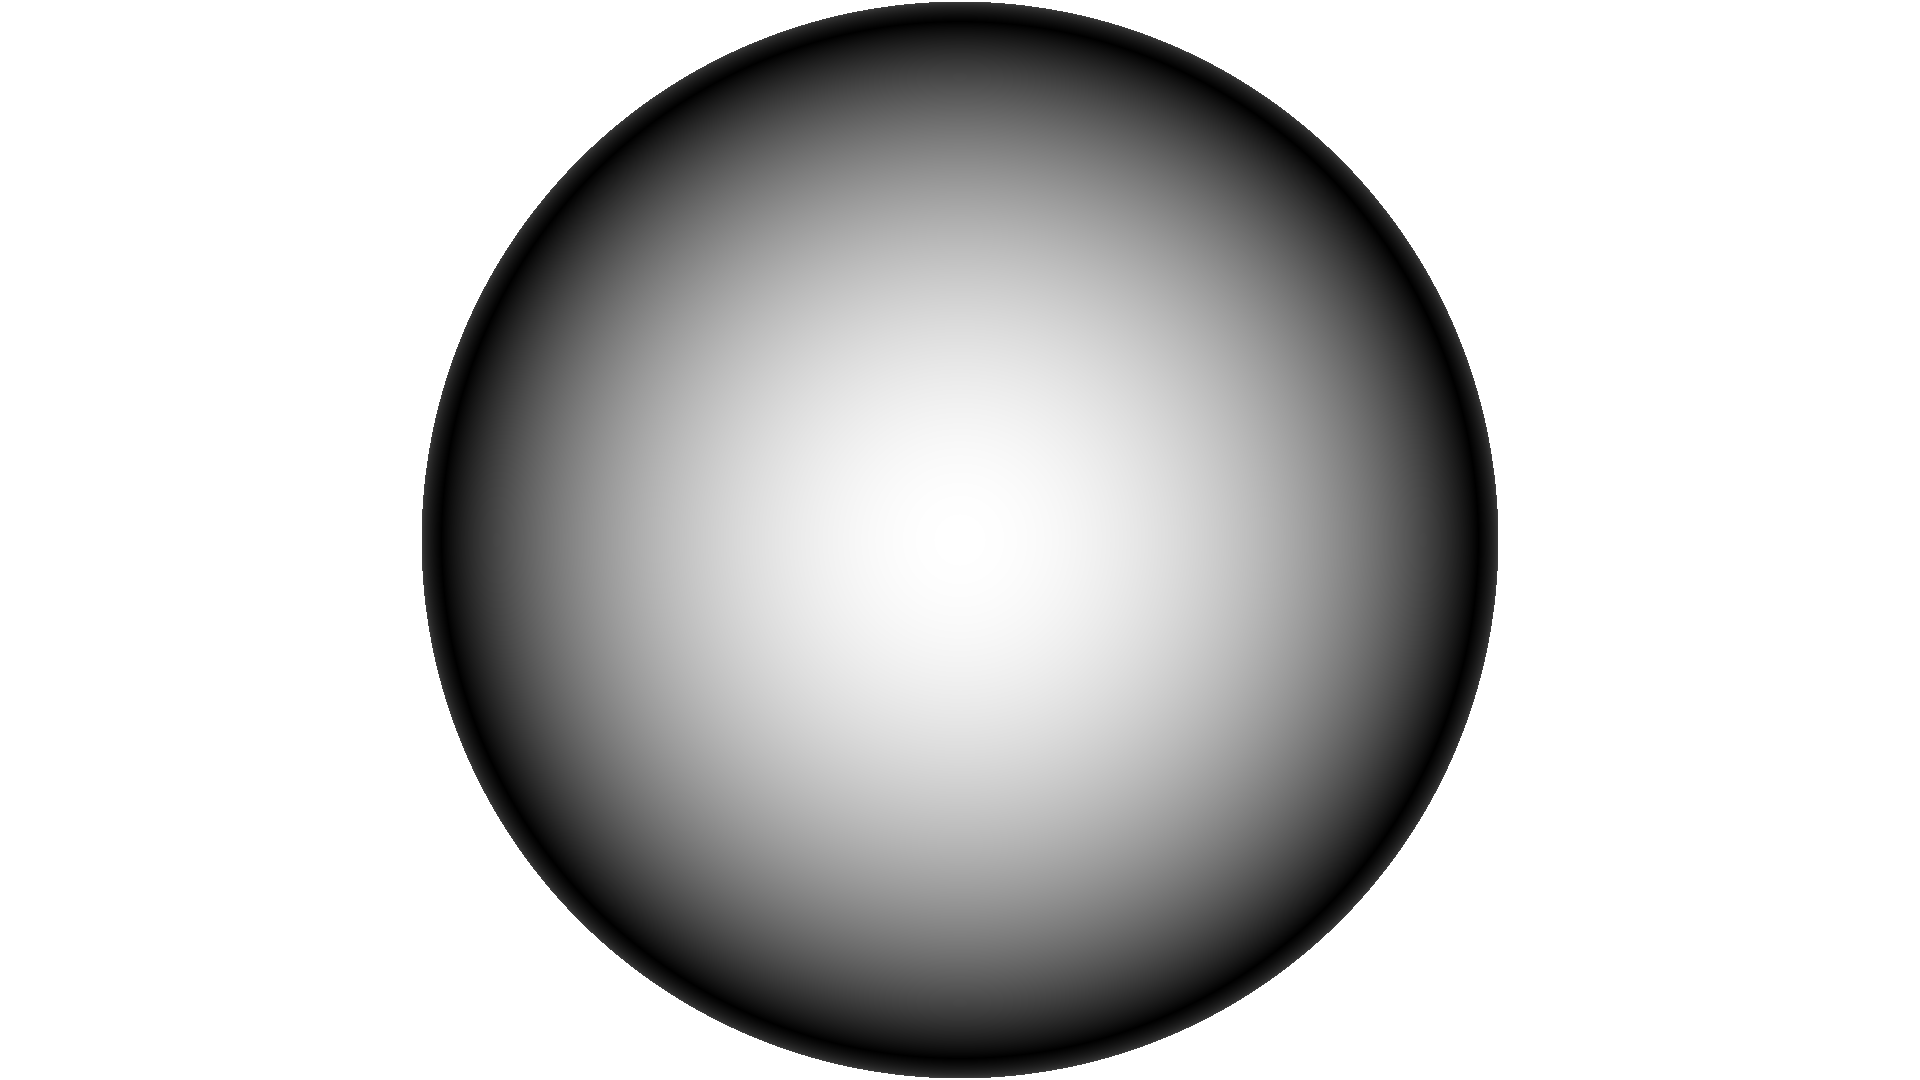
\includegraphics[width=\linewidth]{media/lambert_forward.png}
		\caption*{Eje z.}
	\end{subfigure}%
	\caption{Ilustración de reflexión difusa por cada eje direccional para las caras del vóxel.}
	\label{fig:lambert_dir}
\end{figure}
% section sombreado_de_voxeles (end)

\begin{figure}[H]
	\centering
	\begin{subfigure}[t]{0.49\textwidth}
		\centering
		\captionsetup{justification=centering}
		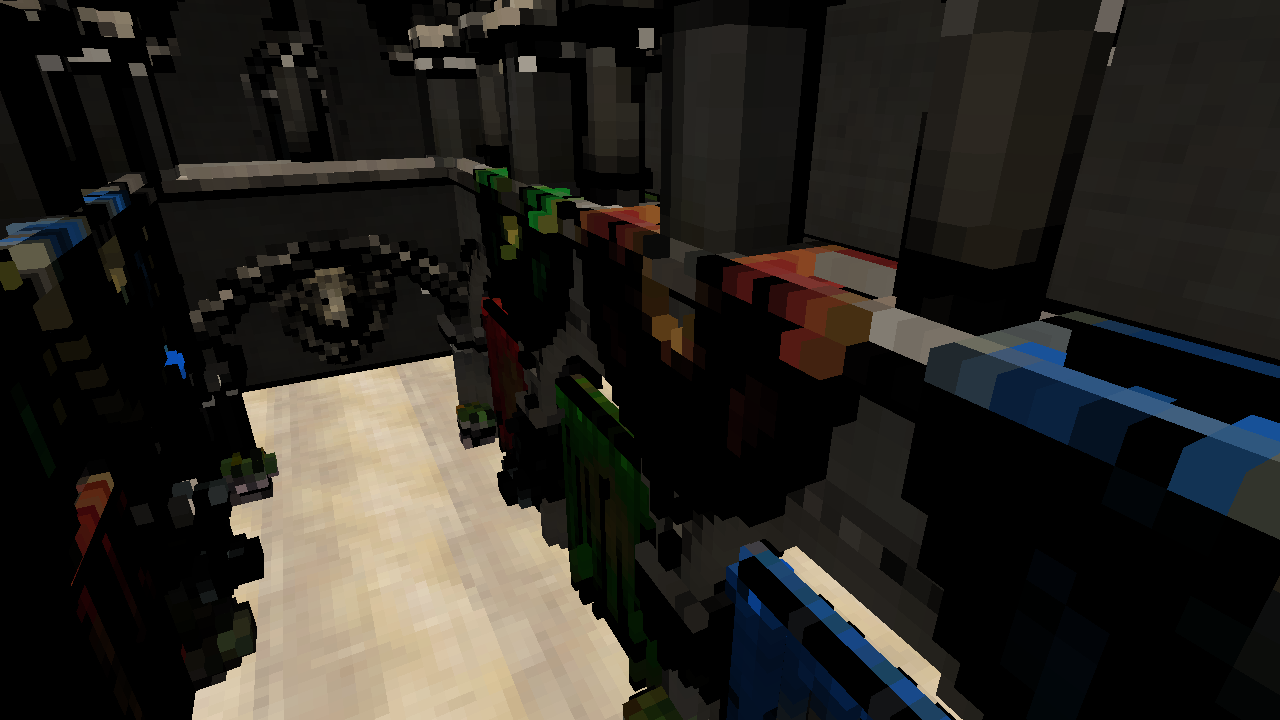
\includegraphics[width=\linewidth]{media/classic_lambert.png}
		\caption*{Lambert..}
	\end{subfigure}%
	\hspace{0.01\textwidth}
	\begin{subfigure}[t]{0.49\textwidth}
		\centering
		\captionsetup{justification=centering}
		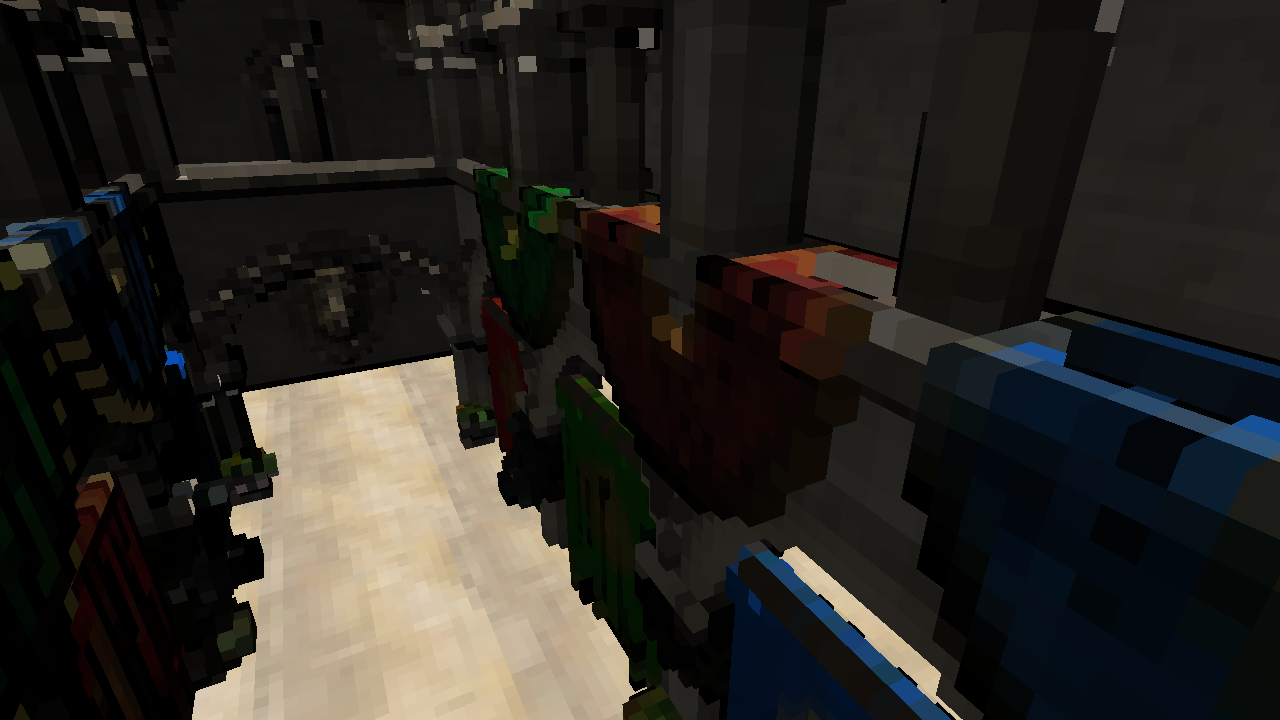
\includegraphics[width=\linewidth]{media/dir_lambert.png}
		\caption*{Lambert Direccional Ponderado.}
	\end{subfigure}%
	\caption{Sombreado difuso de vóxeles utilizando Lambert clásico y Lambert Direccional Ponderado. En la imagen izquierda se puede observar varios vóxeles totalmente negros, estos valores son incorrectos, causados por normales desviadas durante el proceso de voxelización. En la imagen derecha estos vóxeles ahora tienen coloración correcta. También se puede observar que objetos con normales promediadas correctamente como el piso mantienen su sombreado original en ambos modelos.}
	\label{fig:lambert_dir_diff}
\end{figure}

\subsection{Trazado y Mapeo de Sombras sobre el Volumen} % (fold)
\label{sub:trazado_de_sombras_sobre_el_volumen}

Para obtener resultados coherentes durante el trazado de conos es también necesario ocluir los voxeles con sombras generadas a partir de distintas fuentes de luz en escena. Utilizando mapas de luz-vista como en el trabajo de Crassin esto es sencillo ya que los voxeles ocluidos simplemente no reciben iluminacion durante el proceso de captura de la iluminacion directa (seccion \ref{subsub:voxel_capture}).

% subsection trazado_de_sombras_sobre_el_volumen (end)
